\subsubsection{Test af brugerinput}

I dette afsnit vil vi checke om programmet kan modtage og fremstille et billede på baggrund af det input der modtages fra brugeren (krav 1). Nedenstående eksekverings eksempel viser hvordan input modtages fra brugeren.

\begin{lstlisting}
./trace model.ply -o  lamp.pnm -w 800 -h 600 -t 15000 -V -0.5 -H 0.5
\end{lstlisting}

Her ses der at programmet modtager en 3D-fil (model.ply) og at den skal generer et billede (lamp.pnm) som har en 800x600 opløsning. Derudover modtager programmet en farvetemperatur på 15.000 kelvin og får af vide at lampen skal ses fra en vertikal vinkel på -0,5 radianer og en horisontal vinkel på 0,5 radian. En rendering af billedet er vist på \ref{fig:lampe_test1}.

\begin{figure}[H]
  \centering
  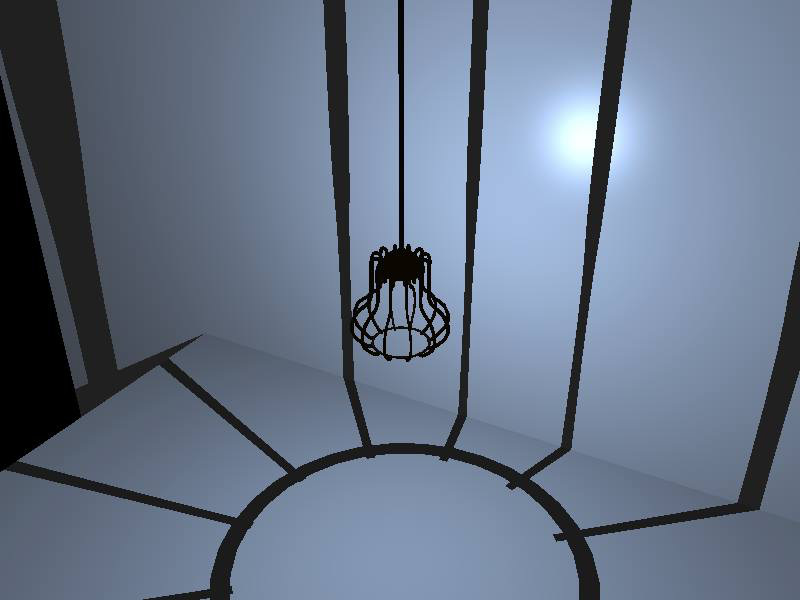
\includegraphics[width=5cm]{lampe_test1}
  \caption{Rendering af et 800x600 billede med en farvetemperatur på 15.000 kelvin samt synsvinklen V -0,5 og H 0,5.}
    \label{fig:lampe_test1}
\end{figure}

Vi vil nu teste om det er muligt at skift farvetemperatur og synsvinkel. For at gøre dette ændres brugerinputtet:
\begin{lstlisting}
./trace model.ply -o  lamp.pnm -w 800 -h 600 -t 1200 -V 0.2
\end{lstlisting}

Farvetemperaturen er nu sat til 1200 kelvin og synsvinklen er sat til en vertikal vinkel på 0.2 radian. Det vi forventer er, at belysningen bliver orange og at billedet ses lige på med en negativ hældning på 0.2 radian.

\begin{figure}[H]
  \centering
  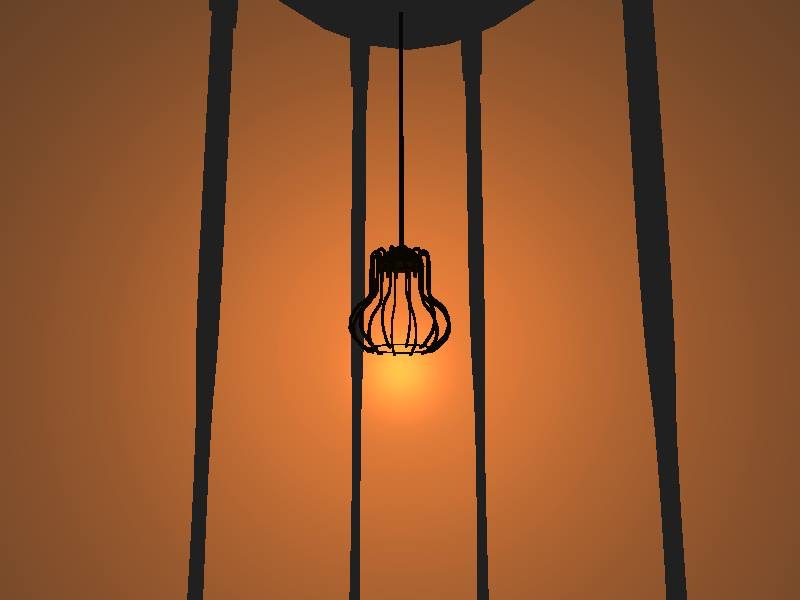
\includegraphics[width=5cm]{lampe_test2}
  \caption{Rendering af et 800x600 billede med en farvetemperatur på 1200 kelvin samt synsvinklen V 0,2}
    \label{fig:lampe_test2}
\end{figure}

Som der ses på billedet er belysningen orange som forventet og lampen er set lige på med en negativ vertikal hældning.

